\documentclass[aspectratio=43,9pt]{beamer}
%
\usepackage{graphicx,tikz}
%
\usetheme{Boadilla}
%
\graphicspath{{./figures/nt6/}}
%
\let\Tiny=\tiny%			% to avoid warnings about font size
%\usepackage{lmodern}%		% alternative method to avoid these warnings
%
\catcode`~=11 % make LaTeX treat tilde (~) like a normal character
\newcommand{\urltilde}{\hbox{~}}
\catcode`~=13 % revert back to treating tilde (~) as an active character
%
% misc commands
\newcommand{\bm}[1]{\mathbf{#1}}
\newcommand{\bs}[1]{\boldsymbol{#1}}
\newenvironment{myitemize}[1]{\vspace{#1}\begin{itemize}\setlength\itemsep{#1}}{\end{itemize}}
%
% pgf markers
\usepgflibrary{plotmarks}
%
\setbeamertemplate{footline}
{
  \leavevmode%
  \hbox{%
  \begin{beamercolorbox}[wd=.8\paperwidth,ht=2.25ex,dp=1ex,left]{author in head/foot}%
    \usebeamerfont{author in head/foot}\hspace*{4em}\inserttitle
  \end{beamercolorbox}%
  \begin{beamercolorbox}[wd=.2\paperwidth,ht=2.25ex,dp=1ex,right]{author in head/foot}%
    \usebeamerfont{author in head/foot}\insertframenumber{} / \inserttotalframenumber\hspace*{1ex}
  \end{beamercolorbox}}%
  \vskip0pt%
}
%
\setbeamertemplate{navigation symbols}{}
%
\setbeamertemplate{frametitle}
{%
	\begin{minipage}{.9\paperwidth}
		\vspace*{1ex}%
		\flushright%
		%\bfseries
		\LARGE%
		\insertframetitle%
	\end{minipage}%
}
%
\setbeamertemplate{title page}{
	\begin{center}
		\vspace*{2ex}
		\usebeamercolor[fg]{frametitle}{%
			\Large%
			Numerical Techniques 2025--2026\\[2ex]
			%
			\LARGE%
			\inserttitle
		}\\[6ex]
		\usebeamercolor[fg]{normal text}{%
			Daan Degrauwe\\[1ex]
			\texttt{daan.degrauwe@meteo.be}\\[4ex]
			Postgraduate Studies in Weather and Climate Modeling\\[1ex]
			Ghent University
		}
	\end{center}
}
%
\newcommand{\ft}[2]{{\textstyle\frac{#1}{#2}}}
%
% increase space around equations
\makeatletter
\g@addto@macro\normalsize{%
	\setlength{\abovedisplayskip}{3ex}%
	\setlength{\belowdisplayskip}{3ex}%
	\setlength{\abovedisplayshortskip}{3ex}%
	\setlength{\belowdisplayshortskip}{3ex}%
}%
\makeatother
%

%
\title{6. Semi-implicit semi-Lagrangian schemes}%
%
%%%%%%%%%%%%%%%%%%%%%%%%%%%%%%%%%%%%%%%%%%%%%%%%%%%%%%%%%%%%%%%%%%%%%%
%
\begin{document}
%
%%%%%%%%%%%%%%%%%%%%%%%%%%%%%%%%%%%%%%%%%%%%%%%%%%%%%%%%%%%%%%%%%%%%%%%%%%%%%%%%%%%%%%%%%%%%%%%%%%%%
%
\begin{frame}[plain]
	\titlepage
\end{frame}
%
%%%%%%%%%%%%%%%%%%%%%%%%%%%%%%%%%%%%%%%%%%%%%%%%%%%%%%%%%%%%%%%%%%%%%%
%
\begin{frame}
	%
	\frametitle{Content}
	%
	\begin{myitemize}{2ex}
		\item Introduction: Eulerian and Lagrangian schemes
			%
		\item Advection equation:
			%
			\begin{myitemize}{1ex}
				\item stability
				\item accurracy
				\item 2D
				\item nonconstant advection speed and forcings
			\end{myitemize}
			%
		\item Shallow water equations
			%
			\begin{myitemize}{1ex}
				\item Semi-Lagrangian linearized SWE
				\item Semi-implicit nonlinear SWE
			\end{myitemize}
			%
	\end{myitemize}
	%
\end{frame}
%
%%%%%%%%%%%%%%%%%%%%%%%%%%%%%%%%%%%%%%%%%%%%%%%%%%%%%%%%%%%%%%%%%%%%%%
%
\begin{frame}
	%
	\frametitle{Eulerian vs. Lagrangian}
	%
	\textbf{Eulerian}:
	%
	\par
	\hspace*{1cm}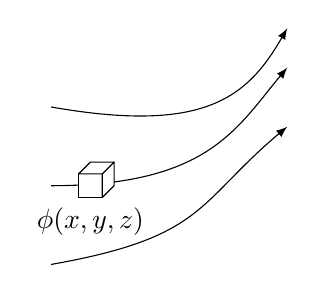
\begin{tikzpicture}[>=latex,x=5mm,y=5mm]
		% stream lines
		\draw[->] (-3,2) .. controls +(-10:4) and +(60:-2) .. (3,4);
		\draw[->] (-3,0) .. controls +(00:4) and +(50:-2) .. (3,3);
		\draw[->] (-3,-2) .. controls +(10:4) and +(40:-3) .. (3,1.5);
		% smallcube on a stream line
		\begin{scope}[x=3mm,y=3mm,xshift=-10mm,yshift=-1.5mm,fill=white,join=round]
			\draw[fill] (-.5,0) -- +(1,0) -- +(1,1) -- +(0,1) -- cycle;
			\draw[fill] (.5,0) -- +(.5,.5) -- +(.5,1.5) -- +(0,1) -- cycle;
			\draw[fill] (-.5,1) -- +(.5,.5) -- +(1.5,.5) -- +(1,0) -- cycle;
			\draw[fill] (0,0) node[below] {$\phi(x,y,z)$};
		\end{scope}
		%
	\end{tikzpicture}\hspace*{1cm}%
	\parbox[b]{.55\textwidth}{
		%
		\begin{equation*}
			\delta \phi = \phi (x,y,z,t+\delta t) -\phi (x,y,z,t)
		\end{equation*}
		%
		The derivative is the partial derivative
		%
		\begin{equation*}
			 \frac{\partial \phi}{\partial t}
		\end{equation*}
		%
	}
	%
\pause
	\par\vspace*{4ex}%
	\textbf{Lagrangian}:
	%
	\par
	\hspace*{1cm}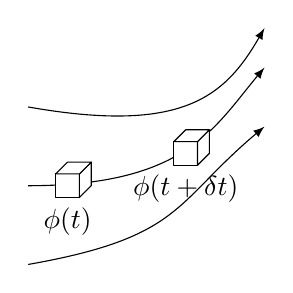
\begin{tikzpicture}[>=latex,x=5mm,y=5mm]
		% stream lines
		\draw[->] (-3,2) .. controls +(-10:4) and +(60:-2) .. (3,4);
		\draw[->] (-3,0) .. controls +(00:4) and +(50:-2) .. (3,3);
		\draw[->] (-3,-2) .. controls +(10:4) and +(40:-3) .. (3,1.5);
		% smallcube on a stream line
		\begin{scope}[x=3mm,y=3mm,xshift=-10mm,yshift=-1.5mm,fill=white,join=round]
			\draw[fill] (-.5,0) -- +(1,0) -- +(1,1) -- +(0,1) -- cycle;
			\draw[fill] (.5,0) -- +(.5,.5) -- +(.5,1.5) -- +(0,1) -- cycle;
			\draw[fill] (-.5,1) -- +(.5,.5) -- +(1.5,.5) -- +(1,0) -- cycle;
			\draw[fill] (0,0) node[below] {$\phi(t)$};
		\end{scope}
		% smallcube further on a stream line
		\begin{scope}[x=3mm,y=3mm,xshift=5mm,yshift=2.6mm,fill=white,join=round]
			\draw[fill] (-.5,0) -- +(1,0) -- +(1,1) -- +(0,1) -- cycle;
			\draw[fill] (.5,0) -- +(.5,.5) -- +(.5,1.5) -- +(0,1) -- cycle;
			\draw[fill] (-.5,1) -- +(.5,.5) -- +(1.5,.5) -- +(1,0) -- cycle;
			\draw[fill] (0,0) node[below] {$\phi(t+\delta t)$};
		\end{scope}
		%
	\end{tikzpicture}\hspace*{1cm}%
	\parbox[b]{.55\textwidth}{
		%
		\begin{equation*}
			\delta \phi = \phi (x + \delta x, y + \delta y, z + \delta z, t + \delta t) -\phi (x,y,z,t)
		\end{equation*}
		%
		The derivative is the total derivative
		%
		\begin{equation*}
			 \frac{D \phi}{D t}
		\end{equation*}
		%
	}
	%
\end{frame}
%
%%%%%%%%%%%%%%%%%%%%%%%%%%%%%%%%%%%%%%%%%%%%%%%%%%%%%%%%%%%%%%%%%%%%%%
%
\begin{frame}
	%
	\frametitle{Eulerian vs. Lagrangian}
	%
	\begin{myitemize}{2ex}
		\item The total derivative is given by
			%
			\begin{equation*}
				\frac{D}{D t} \equiv \frac{\partial}{\partial t} + \frac{D x}{D t} \frac{\partial}{\partial x}
				\quad \text{with} \quad \frac{D x}{D t} = u
			\end{equation*}\vspace*{2mm}
			%
		\item Formulation of the advection equation in Eulerian and Lagrangian shape:
			%
			\begin{equation*}
				 \frac{\partial \psi}{\partial t} + u \frac{\partial \psi}{\partial x} = 0 \qquad\text{or}\qquad \frac{D \psi}{D t} =0
			\end{equation*}
			%
		\item So the time discretisation would be much simpler if we write it in a Lagrangian frame: no \emph{nonlinear} advection term will be present.
			%
	\end{myitemize}
	%
\end{frame}
%
%%%%%%%%%%%%%%%%%%%%%%%%%%%%%%%%%%%%%%%%%%%%%%%%%%%%%%%%%%%%%%%%%%%%%%
%
\begin{frame}
	%
	\frametitle{Eulerian vs. Lagrangian}
	%
	\begin{myitemize}{2ex}
		\item However, in flows that are divergent one may end up with regions that are not well represented by air particles after some time.
			%
	\pause
		\item The solution: use \emph{semi-Lagrangian} trajectories:\\
			%
			\begin{center}
				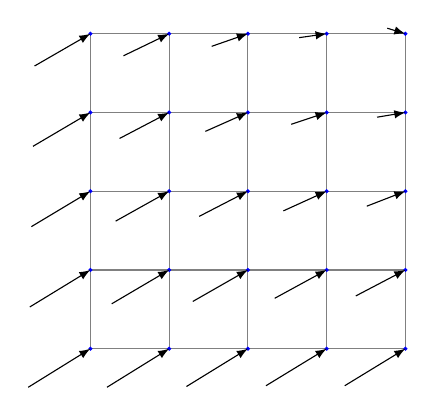
\begin{tikzpicture}[>=latex]
					\draw[step=1,gray] (0,0) grid (4,4);
					\draw [blue, fill=blue] (0,0) node[coordinate] (a) {} circle (.5pt); \draw[<-] (a) -- +(-0.79,-0.49);
					\draw [blue, fill=blue] (1,0) node[coordinate] (a) {} circle (.5pt); \draw[<-] (a) -- +(-0.79,-0.49);
					\draw [blue, fill=blue] (2,0) node[coordinate] (a) {} circle (.5pt); \draw[<-] (a) -- +(-0.78,-0.48);
					\draw [blue, fill=blue] (3,0) node[coordinate] (a) {} circle (.5pt); \draw[<-] (a) -- +(-0.77,-0.47);
					\draw [blue, fill=blue] (4,0) node[coordinate] (a) {} circle (.5pt); \draw[<-] (a) -- +(-0.77,-0.47);
					\draw [blue, fill=blue] (0,1) node[coordinate] (a) {} circle (.5pt); \draw[<-] (a) -- +(-0.77,-0.47);
					\draw [blue, fill=blue] (1,1) node[coordinate] (a) {} circle (.5pt); \draw[<-] (a) -- +(-0.73,-0.43);
					\draw [blue, fill=blue] (2,1) node[coordinate] (a) {} circle (.5pt); \draw[<-] (a) -- +(-0.70,-0.40);
					\draw [blue, fill=blue] (3,1) node[coordinate] (a) {} circle (.5pt); \draw[<-] (a) -- +(-0.66,-0.36);
					\draw [blue, fill=blue] (4,1) node[coordinate] (a) {} circle (.5pt); \draw[<-] (a) -- +(-0.63,-0.33);
					\draw [blue, fill=blue] (0,2) node[coordinate] (a) {} circle (.5pt); \draw[<-] (a) -- +(-0.75,-0.45);
					\draw [blue, fill=blue] (1,2) node[coordinate] (a) {} circle (.5pt); \draw[<-] (a) -- +(-0.68,-0.38);
					\draw [blue, fill=blue] (2,2) node[coordinate] (a) {} circle (.5pt); \draw[<-] (a) -- +(-0.62,-0.32);
					\draw [blue, fill=blue] (3,2) node[coordinate] (a) {} circle (.5pt); \draw[<-] (a) -- +(-0.55,-0.25);
					\draw [blue, fill=blue] (4,2) node[coordinate] (a) {} circle (.5pt); \draw[<-] (a) -- +(-0.49,-0.19);
					\draw [blue, fill=blue] (0,3) node[coordinate] (a) {} circle (.5pt); \draw[<-] (a) -- +(-0.73,-0.43);
					\draw [blue, fill=blue] (1,3) node[coordinate] (a) {} circle (.5pt); \draw[<-] (a) -- +(-0.63,-0.33);
					\draw [blue, fill=blue] (2,3) node[coordinate] (a) {} circle (.5pt); \draw[<-] (a) -- +(-0.54,-0.24);
					\draw [blue, fill=blue] (3,3) node[coordinate] (a) {} circle (.5pt); \draw[<-] (a) -- +(-0.45,-0.15);
					\draw [blue, fill=blue] (4,3) node[coordinate] (a) {} circle (.5pt); \draw[<-] (a) -- +(-0.36,-0.06);
					\draw [blue, fill=blue] (0,4) node[coordinate] (a) {} circle (.5pt); \draw[<-] (a) -- +(-0.71,-0.41);
					\draw [blue, fill=blue] (1,4) node[coordinate] (a) {} circle (.5pt); \draw[<-] (a) -- +(-0.58,-0.28);
					\draw [blue, fill=blue] (2,4) node[coordinate] (a) {} circle (.5pt); \draw[<-] (a) -- +(-0.46,-0.16);
					\draw [blue, fill=blue] (3,4) node[coordinate] (a) {} circle (.5pt); \draw[<-] (a) -- +(-0.35,-0.05);
					\draw [blue, fill=blue] (4,4) node[coordinate] (a) {} circle (.5pt); \draw[<-] (a) -- +(-0.23,0.07);
				\end{tikzpicture}
				\hspace*{1cm}
				\raisebox{3cm}{\parbox{.35\textwidth}{%
					Choose departure points such that the trajectories arrive in the grid points of the model at the end of the time step.\\[5pt]
					%
					The departure points are recalculated \emph{every time step}!
				}}
			\end{center}
			%
	\end{myitemize}
	%
\end{frame}
%
%%%%%%%%%%%%%%%%%%%%%%%%%%%%%%%%%%%%%%%%%%%%%%%%%%%%%%%%%%%%%%%%%%%%%%
%
\begin{frame}
	%
	\frametitle{Advection equation}
	%
	\begin{myitemize}{2ex}
		\item The 1D advection equation \emph{with constant advection speed $U$} is discretized in the semi-Lagrangian form as
			%
			\begin{equation*}
				\frac{\phi (x_j, t^{n+1}) - \phi (\tilde x_j, t^n)}{\Delta t} = 0
			\end{equation*}
			%
			with the \emph{departure point} given by
			%
			\begin{equation*}
				\tilde x_j = x_j -U \Delta t
			\end{equation*}
			%
		\item Define
			%
			\begin{equation*}
				p = \left\lfloor \frac{U \Delta t}{\Delta x} \right\rfloor
			\end{equation*}
			%
			with $\lfloor z\rfloor$ the integer part of $z$, then
			%
			\begin{equation*}
				x_{j-p-1} \le\tilde x_j \le x_{j-p}
			\end{equation*}
			%
	\end{myitemize}
	%
\end{frame}
%
%%%%%%%%%%%%%%%%%%%%%%%%%%%%%%%%%%%%%%%%%%%%%%%%%%%%%%%%%%%%%%%%%%%%%%
%
\begin{frame}
	%
	\frametitle{Advection equation}
	%
	\begin{myitemize}{2ex}
		\item Now, define
			%
			\begin{equation*}
				\alpha = \frac{x_{j-p} - \tilde x_j^n}{\Delta x}
			\end{equation*}
			%
		\item Note that by construction, $0 \le \alpha \le 1$, because $x_{j-p-1} \le \tilde x_j^n \le x_{j-p}$\vspace*{10mm}
			%
	\end{myitemize}
	%
	\begin{center}
		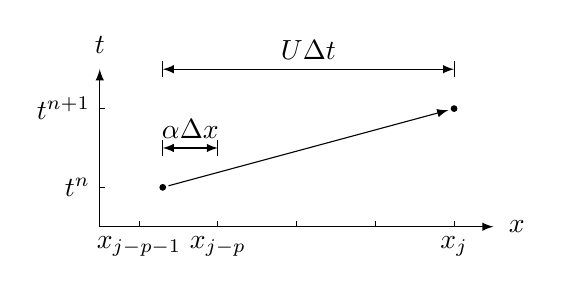
\begin{tikzpicture}[>=latex]
			% x axis
			\draw[->] (-.5,0) -- +(5,0) node[right=2pt] {$x$};
			\draw (0,0) -- +(0,2pt) node[below=2pt] {$x_{j-p-1}$}
				 (1,0) -- +(0,2pt) node[below=2pt] {$x_{j-p}$}
				 (2,0) -- +(0,2pt)
				 (3,0) -- +(0,2pt)
				 (4,0) -- +(0,2pt) node[below=2pt] {$x_{j}$};
			% y axis
			\draw[->] (-.5,0) -- +(0,2) node[above=2pt] {$t$};
			\draw (-.5,.5) -- +(2pt,0) node[left=2pt] {$t^{n}$}
				 (-.5,1.5) -- +(2pt,0) node[left=2pt] {$t^{n+1}$};
			% arrival and departure points
			\draw[fill] (4,1.5) circle (1pt);
			\draw[fill] (0.3,0.5) circle (1pt);
			% trajectory
			\draw[<-] (3.926,1.48) -- (.374,.52);
			% annotations
			\draw[<->] (.3,1) -- (1,1) node[pos=.5,above] {$\alpha\Delta x$};
			\draw (.3,.9) -- +(0,.2) (1,.9) -- +(0,.2);
			\draw[<->] (.3,2) -- (4,2) node[pos=.5,above] {$U\Delta t$};
			\draw (.3,1.9) -- +(0,.2) (4,1.9) -- +(0,.2);
		\end{tikzpicture}
	\end{center}
	%
\end{frame}
%
%%%%%%%%%%%%%%%%%%%%%%%%%%%%%%%%%%%%%%%%%%%%%%%%%%%%%%%%%%%%%%%%%%%%%%
%
\begin{frame}
	%
	\frametitle{Advection equation}
	%
	\begin{myitemize}{2ex}
		\item Next, we have to approximate $\phi$ in $\tilde x_j^n$, e.g. by a linear interpolation
			%
			\begin{equation*}
				\phi ( \tilde x_j^n, t^n) = (1-\alpha) \phi^n_{j-p} + \alpha \phi_{j-p-1}^n
			\end{equation*}
			%
		\item The advection equation then becomes
			%
			\begin{equation*}
				\frac{\phi^{n+1}_j-\phi(\tilde x_j^n,t^n)}{\Delta t} = 0
			\end{equation*}
			%
			or
			%
			\begin{equation*}
				\phi^{n+1}_j = \phi(\tilde x_j^n,t^n) = (1-\alpha) \phi^n_{j-p} + \alpha \phi_{j-p-1}^n
			\end{equation*}
			%
	\pause
		\item \textbf{Note 1}: this is an \emph{explicit} scheme: values at the next timestep $n+1$ only appear on the left-hand side.
			%
		\item \textbf{Note 2}: this is very similar to the upstream scheme; even identical if $p=0$.
	\end{myitemize}
	%
\end{frame}
%
%%%%%%%%%%%%%%%%%%%%%%%%%%%%%%%%%%%%%%%%%%%%%%%%%%%%%%%%%%%%%%%%%%%%%%
%
\begin{frame}
	%
	\frametitle{Advection equation: Stability}
	%
	\begin{myitemize}{2ex}
		\item Von Neumann analysis on a solution of the form $\phi_j^n = A_k^n e^{i(kj \Delta x)}$
			%
			\begin{equation*}
				A_k = \left[ 1 - \alpha \left( 1 - e^{-i k \Delta x} \right) \right] e^{-i k p \Delta x}
			\end{equation*}
			%
			or
			%
			\begin{equation*}
				| A_k |^2 = 1 - 2 \alpha (1-\alpha) ( 1 -\cos k \Delta x )
			\end{equation*}
			%
			then the condition for stability becomes
			%
			\begin{equation*}
				0 \le \alpha \le 1
			\end{equation*}
			%
			which is \textbf{always} satisfied!
			%
	\end{myitemize}
	%
\end{frame}
%
%%%%%%%%%%%%%%%%%%%%%%%%%%%%%%%%%%%%%%%%%%%%%%%%%%%%%%%%%%%%%%%%%%%%%%
%
\begin{frame}
	%
	\frametitle{Advection equation: accuracy}
	%
	\begin{myitemize}{2ex}
		\item Consider the Taylor expansion of
			%
			\begin{equation*}
				\frac{ \phi_j^{n+1} - \left[ (1-\alpha) \phi^n_{j-p} + \alpha \phi_{j-p-1}^n \right]} {\Delta t} = 0
			\end{equation*}
			%
			around the departure point $(\tilde x_j^n, t^n)$. Then
			%
			\begin{equation*}
				\frac{ \psi_j^{n+1} - \left[ (1-\alpha) \psi^n_{j-p} + \alpha \psi_{j-p-1}^n\right]}{\Delta t}
					\approx - \ft12 \alpha (1-\alpha) \frac{\Delta x^2}{\Delta t} \left. \frac{\partial^2 \psi}{\partial x^2} \right|_{\tilde x_j^n}
			\end{equation*}
			%
		\item It seems that this could not be consistent if we take the limit $\Delta t \rightarrow 0$ faster than $\Delta x^2\rightarrow 0$.
			%
\pause
		\item However, if the Courant number $U \Delta t / \Delta x$ becomes smaller than $1$, then $\alpha = U \Delta t / \Delta x$. Using $\partial^2 \psi / \partial t^2 = U^2 \partial^2 \psi / \partial x^2$, the error becomes
			%
			\begin{equation*}
				\ft12 \Delta t \frac{\partial^2 \psi}{\partial t^2} - \ft12 U \Delta x \frac{\partial^2 \psi}{\partial x^2} \qquad \text{which is first order}
			\end{equation*}
			%
	\end{myitemize}
	%
\end{frame}
%
%%%%%%%%%%%%%%%%%%%%%%%%%%%%%%%%%%%%%%%%%%%%%%%%%%%%%%%%%%%%%%%%%%%%%%
%
\begin{frame}
	%
	\frametitle{Advection equation: Higher order}
	%
	\begin{myitemize}{4ex}
		\item Quadratic interpolation:
			%
			\begin{equation*}
				\phi (\tilde x_j^n, t^n) = \ft12 \alpha (1+\alpha) \phi_{j-p-1}^n + (1 - \alpha^2) \phi_{j-p}^n + \ft12 \alpha (1-\alpha) \phi_{j-p+1}^n
			\end{equation*}
			%
			with $p + \alpha = U \Delta t$ but $p$ such that $| \alpha | \le \ft12$.
			%
			\par\vspace*{2ex}
			This yields $O [ \Delta x^3 / \Delta t]$ which gives a second-order accurate scheme.
			%
		\item The cubic interpolation with $p + \alpha = U \Delta t$ and $0\leq\alpha\leq1$ and
			%
			\begin{align*}
				\phi ( \tilde x_j^n, t^n ) =& - \ft16 (1+\alpha)\alpha(1-\alpha) \phi^n_{j-p-2} + \ft12 (1+\alpha)\alpha(2-\alpha) \phi_{j-p-1}^n \\
					& + \ft12 (1+\alpha)(1-\alpha)(2-\alpha) \phi_{j-p}^n - \ft16 \alpha(1-\alpha)(2-\alpha) \phi_{j-p+1}^n
			\end{align*}
			%
			yields third-order accuracy.
			%
	\end{myitemize}
	%
\end{frame}
%
%%%%%%%%%%%%%%%%%%%%%%%%%%%%%%%%%%%%%%%%%%%%%%%%%%%%%%%%%%%%%%%%%%%%%%
%
\begin{frame}
	%
	\frametitle{Advection equation: 2D}
	%
	\begin{myitemize}{2ex}
		\item In 2 dimensions,
			%
			\begin{equation*}
				\frac{D\psi}{D t}=\frac{\partial \psi}{\partial t}+U\frac{\partial \psi}{\partial x}+V\frac{\partial \psi}{\partial y} = 0
			\end{equation*}
			%
			is discretized as
			%
			\begin{equation*}
				\frac{\phi (x_{j_x}, y_{j_y}, t^{n+1}) - \phi (\tilde x_{j_x,j_y}, \tilde y_{j_x,j_y}, t^n ) } {\Delta t} = 0
			\end{equation*}
			%
			with $(\tilde x_{j_x,j_y}, \tilde y_{j_x,j_y}$) the departure point and $(x_{j_x}, y_{j_y})$ the arrival point.
			%
		\item The definition of $p$ and $\alpha$ is similar to the 1D case:
			%
			\begin{align*}
				p &= \left\lfloor \frac{U \Delta t}{\Delta x} \right\rfloor & \alpha &	= \frac{U \Delta t }{\Delta x}-p \\
				q &= \left\lfloor \frac{V \Delta t}{\Delta y} \right\rfloor	&	\beta &	= \frac{V \Delta t }{\Delta y}-q
			\end{align*}
			%
			with $0\le\alpha,\beta\le1$
			%
	\end{myitemize}
	%
\end{frame}
%
%%%%%%%%%%%%%%%%%%%%%%%%%%%%%%%%%%%%%%%%%%%%%%%%%%%%%%%%%%%%%%%%%%%%%%
%
\begin{frame}
	%
	\frametitle{Advection equation: 2D}
	%
	\begin{myitemize}{2ex}
		\item On a quadratic \emph{stencil}:
			%
			\begin{center}
				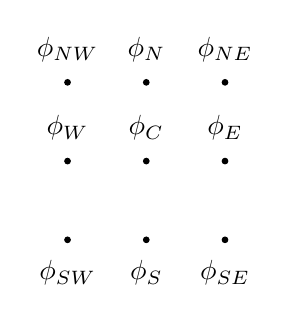
\begin{tikzpicture}[x=10mm,y=10mm]
					\draw[fill] (-1,1) circle (1pt) node[above=4pt] {$\phi_{NW}$};
					\draw[fill] (0,1) circle (1pt) node[above=4pt] {$\phi_N$};
					\draw[fill] (1,1) circle (1pt) node[above=4pt] {$\phi_{NE}$};
					\draw[fill] (-1,0) circle (1pt) node[above=4pt] {$\phi_{W}$};
					\draw[fill] (0,0) circle (1pt) node[above=4pt] {$\phi_C$};
					\draw[fill] (1,0) circle (1pt) node[above=4pt] {$\phi_{E}$};
					\draw[fill] (-1,-1) circle (1pt) node[below=4pt] {$\phi_{SW}$};
					\draw[fill] (0,-1) circle (1pt) node[below=4pt] {$\phi_S$};
					\draw[fill] (1,-1) circle (1pt) node[below=4pt] {$\phi_{SE}$};
				\end{tikzpicture}
			\end{center}
			%
			\begin{align*}
				\tilde \phi^{n+1}\, =\, & \ft12\alpha(1+\alpha)\left[\ft12\beta(1+\beta) \phi_{SW}^n + ( 1- \beta^2) \phi_W^n - \ft12\beta(1-\beta) \phi_{NW}^n\right] \\
						& + (1-\alpha^2)       \left[\ft12\beta(1+\beta) \phi_{S}^n  + ( 1- \beta^2) \phi_C^n - \ft12\beta(1-\beta) \phi_{N}^n \right] \\
						&-\ft12\alpha(1-\alpha)\left[\ft12\beta(1+\beta) \phi_{SE}^n + ( 1- \beta^2) \phi_E^n - \ft12\beta(1-\beta) \phi_{NE}^n\right]
			\end{align*}
			%
			\par
			This is second-order accurate.
	\end{myitemize}
	%
\end{frame}
%
%%%%%%%%%%%%%%%%%%%%%%%%%%%%%%%%%%%%%%%%%%%%%%%%%%%%%%%%%%%%%%%%%%%%%%
%
\begin{frame}
	%
	\frametitle{Advection equation: 2D}
	%
	\begin{myitemize}{2ex}
		\item Ritchie et al. (1995): use cubic interpolation on a 12-point stencil where the corner points are neglected:
			%
			\begin{center}\vspace*{4ex}
				\begin{tikzpicture}
					\draw[fill] (-1,0) circle (1pt) (-1,1) circle (1pt);
					\draw[fill] (0,-1) circle (1pt) (0,0) circle (1pt) (0,1) circle (1pt) (0,2) circle (1pt);
					\draw[fill] (1,-1) circle (1pt) (1,0) circle (1pt) (1,1) circle (1pt) (1,2) circle (1pt);
					\draw[fill] (2,0) circle (1pt) (2,1) circle (1pt);
					\draw (0.4,0.7) node [below right] {$\tilde x$} +(1.5pt,1.5pt) -- +(-1.5pt,-1.5pt) + (-1.5pt,1.5pt) -- +(1.5pt,-1.5pt);
				\end{tikzpicture}
			\end{center}\vspace*{4ex}
			%
			gives unconditionally stable schemes.
			%
	\end{myitemize}
\end{frame}
%
%%%%%%%%%%%%%%%%%%%%%%%%%%%%%%%%%%%%%%%%%%%%%%%%%%%%%%%%%%%%%%%%%%%%%%
%
\begin{frame}
	%
	\frametitle{Variable velocity}
	%
	\begin{myitemize}{2ex}
		\item If the velocity is not constant, the calculation of the departure point is no longer trivial/exact.
			%
		\item The truncation error consists of two terms: an error on the departure point $+$ an error on the interpolation:\vspace*{-1pt}
			%
			\begin{equation*}
				\frac{1}{\Delta t}\left(\psi_j^{n+1} - \psi_d\right) + \frac{1}{\Delta t} \left( \psi_d - \sum_{k=-r}^s \beta_k \psi_{j-p+k}^n\right)
			\end{equation*}
			%
			with $\psi_d = \psi (\tilde x_j^n, t^n)$ and $\beta_k$ the coefficients of the interpolation.
			%
		\item Suppose the departure point is computed as follows:
			%
			\begin{equation*}
				\tilde x_j^n = x^{n+1} - u(x^{n+1}, t^n ) \Delta t
			\end{equation*}
			%
			then one can show (Taylor expansion!) that
			%
			\begin{equation*}
				\psi_j^{n+1} = \psi_d + O [ \Delta t^2 ]
			\end{equation*}
			%
	\end{myitemize}
	%
\end{frame}
%
%%%%%%%%%%%%%%%%%%%%%%%%%%%%%%%%%%%%%%%%%%%%%%%%%%%%%%%%%%%%%%%%%%%%%%
%
\begin{frame}
	%
	\frametitle{Variable velocity}
	%
	\begin{myitemize}{2ex}
		\item So the truncation error due to the calculation of the departure point is
			%
			\begin{equation*}
				\frac{\psi_j^{n+1} - \psi_d}{\Delta t} = O [ \Delta t ]
			\end{equation*}
			%
		\item Hence this method is first order accurate: $O [ \Delta t ]$.
			%
	\end{myitemize}
	%
\end{frame}
%
%%%%%%%%%%%%%%%%%%%%%%%%%%%%%%%%%%%%%%%%%%%%%%%%%%%%%%%%%%%%%%%%%%%%%%
%
\begin{frame}
	%
	\frametitle{Variable velocity: midpoint method}
	%
	\begin{myitemize}{2ex}
		\item Estimating $\tilde x$ by a midpoint method:
			%
			\begin{align*}
				x_* &= x^{n+1} - u(x^{n+1}, t^n ) \Delta t \textcolor{red}{/2} \\
					\tilde x_j^n &= x^{n+1} - u(x_*, t^{n+\ft12} ) \Delta t
			\end{align*}
			%
			This scheme is second-order accurate.
			%
			\begin{center}
				\begin{tikzpicture}[>=latex,y=6mm]
					\draw[->] (0,0) -- (5,0) node [below right] {$x$} ;
					\draw[->] (0,0) -- (0,5) node [above left] {$t$};
					\draw[dashed] (0,1) node [left] {$n$} -- (4.5,1);
					\draw[dashed] (0,3) node [left] {$n+1$} -- (4.5,3);
					\draw[fill] (1,1) circle (1pt);
					\draw[fill] (4,3) circle (1pt);
					\draw (1,1) node [below] {$\tilde x_j$} -- (4,3) node [above right] {$x_j$};
					\draw[line width=1pt] (2.5,2) node [below right] {$x_*$} +(-1.5pt,-1.5pt) -- +(1.5pt,1.5pt) +(-1.5pt,1.5pt) -- +(1.5pt,-1.5pt);
				\end{tikzpicture}
			\end{center}
			%
		\item But how do we determine $u(x_*, t^{n+\ft12})$?
			%
	\end{myitemize}
	%
\end{frame}
%
%%%%%%%%%%%%%%%%%%%%%%%%%%%%%%%%%%%%%%%%%%%%%%%%%%%%%%%%%%%%%%%%%%%%%%
%
\begin{frame}
	%
	\frametitle{Variable velocity: midpoint method}
	%
	\begin{myitemize}{1ex}
		\item In fact it would be best to compute the wind at $t^{n+\ft12}$ by interpolating between $t^n$ and $t^{n+1}$.
		\item This is possible for passive tracers (e.g. pollutants).
		\item But for NWP it is not feasible: wind itself is an forecasted field, which is advected by itself!
		\item<2-> Solution: \emph{time extrapolation}\\[2pt]
			%
	\end{myitemize}
	%
	\begin{center}
		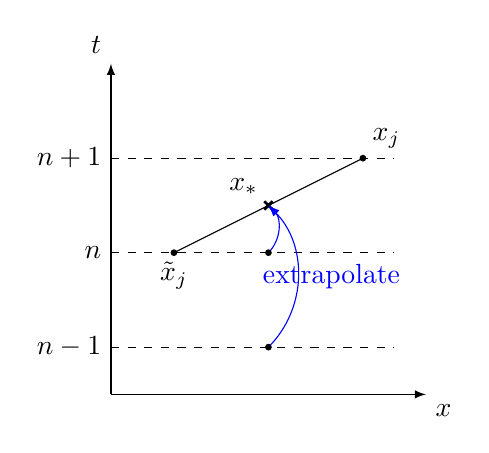
\begin{tikzpicture}[>=latex,y=6mm,x=8mm]
			\draw[->] (0,0) -- (5,0) node [below right] {$x$} ;
			\draw[->] (0,0) -- (0,7) node [above left] {$t$};
			\draw[dashed] (0,3) node [left] {$n$} -- (4.5,3);
			\draw[dashed] (0,5) node [left] {$n+1$} -- (4.5,5);
			\draw[fill] (1,3) circle (1pt);
			\draw[fill] (4,5) circle (1pt);
			\draw (1,3) node [below] {$\tilde x_j$} -- (4,5) node [above right] {$x_j$};
			\draw[line width=1pt] (2.5,4) node [above left] {$x_*$} +(-1.5pt,-1.5pt) -- +(1.5pt,1.5pt) +(-1.5pt,1.5pt) -- +(1.5pt,-1.5pt);
\only<2->{%
			\draw [blue,->] (2.5,1) to[out=45,in=-45] (2.5,4);
			\draw [blue,->] (2.5,3) to[out=45,in=-45] (2.5,4);
			\draw (3.5,2.5) node [rotate=0,blue] {extrapolate};			
			\draw[fill] (2.5,1) circle (1pt);
			\draw[fill] (2.5,3) circle (1pt);
			\draw[dashed] (0,1) node [left] {$n-1$} -- (4.5,1);
		}%
		\end{tikzpicture}%
		%
\onslide<2->{%
		\hspace*{5mm}\raisebox{2cm}{\parbox{5 cm}{
			$u(x_*,t^{n+\ft12})$ is obtained by extrapolating from $t^{n-1}$ and $t^n$:
			%
			\begin{equation*}
				u ( t^{n+\ft12} ) = \ft32 u(t^n) - \ft12 u(t^{n-1})
			\end{equation*}
			%
			which is then linearly interpolated in space to $x_*$.
		}}}
	\end{center}
	%
\end{frame}
%
%%%%%%%%%%%%%%%%%%%%%%%%%%%%%%%%%%%%%%%%%%%%%%%%%%%%%%%%%%%%%%%%%%%%%%
%
\begin{frame}
	%
	\frametitle{Variable velocity: midpoint method}
	%
	\begin{myitemize}{4ex}
		\item The estimated velocity is second-order in time and in space:
			%
			\begin{equation*}
				u (x_*, t^{n+\ft12}) = u_* + O [ \Delta x^2 ] + O [ \Delta t^2 ]
			\end{equation*}
			%
		\item This adds a term of order $O [ \Delta t \Delta x^2 ] + O [ \Delta t^3 ]$ in the estimation of the departure point.
			%
		\item So there is a $O [ \Delta x^2 ] + O [ \Delta t^2 ]$ contribution in the semi-Lagrangian solution.
			%
	\end{myitemize}
	%
\end{frame}
%
%%%%%%%%%%%%%%%%%%%%%%%%%%%%%%%%%%%%%%%%%%%%%%%%%%%%%%%%%%%%%%%%%%%%%%
%
\begin{frame}
	%
	\frametitle{Variable velocity: midpoint method}
	%
	In practice the algorithm gets the following form:
	%
	\begin{enumerate}
		%
		\item estimate the midpoint
			%
			\[x_*= x^{n+1} - u(x^{n+1}, t^n ) \Delta t/2 \]
			%
		\item linearly interpolate the current velocity and the previous velocity to this point:
			%
			\[u(t^n,x^*),\quad u(t^{n-1},x^*)\]
			%
		\item compute the velocity at the midpoint by extrapolating in time
			%
			\[u_*=u ( t^{n+\ft12}, x^* ) = \ft32 u(t^n,x^*) - \ft12 u(t^{n-1},x^*)\]
			%
		\item compute the departure point $\tilde x_j^n = x^{n+1} - u_* \Delta t$
			%
		\item evaluate $\phi ( \tilde x_j^n, t^n)$ using a quadratic interpolation
			%
		\item set $\phi_j^{n+1}$ equal to this.
			%
	\end{enumerate}
	%
\end{frame}
%
%%%%%%%%%%%%%%%%%%%%%%%%%%%%%%%%%%%%%%%%%%%%%%%%%%%%%%%%%%%%%%%%%%%%%%
%
\begin{frame}
	%
	\frametitle{Variable velocity: iterative method}
	%
	\begin{myitemize}{2ex}
		\item One may invent more accurate schemes, for instance by solving the implicit equation
			%
			\begin{equation*}
				\tilde x_j^n = x_j - u \left( \ft12 (x_j + \tilde x_j^n ), t^{n+\ft12}\right)\Delta t
			\end{equation*}
			%
			iteratively.
			%
		\item The midpoint method that we have discussed is actually an example of this.	
			%
	\end{myitemize}
	%
\end{frame}
%
%%%%%%%%%%%%%%%%%%%%%%%%%%%%%%%%%%%%%%%%%%%%%%%%%%%%%%%%%%%%%%%%%%%%%%
%
\begin{frame}
	%
	\frametitle{Forcing terms}
	%
	\begin{myitemize}{3ex}
		\item Let us consider the prototype problem (oscillation $+$ diffusion)
			%
			\begin{equation*}
				\frac{D \psi}{D t} = S = i \omega \psi + \lambda \psi \qquad \text{with} \qquad \frac{D}{Dt} = \frac{\partial}{\partial t} + U \frac{\partial}{\partial x}
			\end{equation*}
			%
		\item The exact solution
			%
			\begin{equation*}
				\psi(x,t) = f (x - U t) e^{(i \omega + \lambda) t}
			\end{equation*}
			%
			is non amplifying for $\lambda \le 0$.
			%
		\item This can be discretized in a semi-Lagrangian way as follows:
			%
			\begin{equation*}
				\frac{\phi (x_j, t^{n+1}) - \phi (\tilde x_j^{n}, t^{n})}{2 \Delta t} =  \ft12 S(x_j, t^{n+1} )+\ft12 S(\tilde x_j^n,t^n)
			\end{equation*}
			%
	\end{myitemize}
	%
\end{frame}
%
%%%%%%%%%%%%%%%%%%%%%%%%%%%%%%%%%%%%%%%%%%%%%%%%%%%%%%%%%%%%%%%%%%%%%%
%
\begin{frame}
	%
	\frametitle{Forcing terms}
	%
	\begin{myitemize}{2ex}
		\item Stability with Von Neumann analysis
			%
			\begin{equation*}
				A_k e^{i k j \Delta x} - e^{ik (j \Delta x - s)} = \ft12 (\tilde \lambda + i \tilde \omega ) \left( A_k e^{ikj \Delta x} + e^{ik (j \Delta x -s)}\right)
			\end{equation*}
			%
			with $\tilde \lambda = \lambda \Delta t$, $\tilde \omega = \omega \Delta t$ and $s=x_j-\tilde x_j$.
			%
			\begin{equation*}
				| A_k |^2 = \left| A_k e^{iks} \right|^2 = \frac{ \left( 1 + \ft12 \tilde \lambda  \right)^2 + \ft14 \tilde \omega^2 }{ \left( 1 - \ft12 \tilde \lambda \right)^2 + \ft14 \tilde \omega^2 }
			\end{equation*}
			%
			which is always smaller than 1 for $\lambda \le 0$. Note that this is even independent of the advection $U$!
			%
	\end{myitemize}
\end{frame}
%
%%%%%%%%%%%%%%%%%%%%%%%%%%%%%%%%%%%%%%%%%%%%%%%%%%%%%%%%%%%%%%%%%%%%%%
%
\begin{frame}
	%
	\frametitle{Linear shallow-water equations}
	%
	\begin{myitemize}{2ex}
		\item Let us consider the shallow-water equations
			%
			\begin{align*}
				\frac{D u}{D t} &= -g \frac{\partial h}{\partial x} \\
				\frac{D h}{D t} &= - H \frac{\partial u}{\partial x}
			\end{align*}
			%
		\item The advection is treated with a semi-Lagrangian scheme; the other terms are linearized.
			%
		\item Consider a leapfrog time integration:
			%
			\begin{align*}
				\frac{u^+ - u^-}{2 \Delta t} &= -g \left(
				\frac{\partial h}{\partial x}
				\right)^0
				\\
				\frac{h^+-h^-}{2 \Delta t} &= - H
				\left(
				\frac{\partial u}{\partial x}
				\right)^0 
			\end{align*}
			%
			Note that the superscripts $+$, $0$ and $-$ also mean evaluation in $x_j$, $\tilde x_j$ and $\check x_j$
			%
	\end{myitemize}
	%
\end{frame}
%
%%%%%%%%%%%%%%%%%%%%%%%%%%%%%%%%%%%%%%%%%%%%%%%%%%%%%%%%%%%%%%%%%%%%%%
%
\begin{frame}
	%
	\frametitle{Linear shallow-water equations}
	%
	\begin{myitemize}{2ex}
		\item Stability analysis with von Neumann method: difficult because it would lead to a quadratic matrix equation:
			%
			\begin{myitemize}{1ex}
				\item 3 timelevel $\Rightarrow$ quadratic
				\item system of 2 equations $\Rightarrow$ $2\times 2$ amplification matrix
			\end{myitemize}
			%
		\item However, we can reformulate the scheme as a 2-timelevel system of 4 equations.
			%
			\par\vspace*{2ex}
			Let
			%
			\begin{equation*}
				\bm v^t=\left(\begin{array}{cccc}u^t & h^t & u^{t-\Delta t} & h^{t-\Delta t}\end{array}\right)^T,
			\end{equation*}
			%
			then
			%
			\begin{equation*}
				\bm v^{t+\Delta t}=\left(\begin{array}{cccc}u^{t+\Delta t} & h^{t +\Delta t} & u^{t} & h^{t}\end{array}\right)^T,
			\end{equation*}
			%
	\end{myitemize}
	%
\end{frame}
%
%%%%%%%%%%%%%%%%%%%%%%%%%%%%%%%%%%%%%%%%%%%%%%%%%%%%%%%%%%%%%%%%%%%%%%
%
\begin{frame}
	%
	\frametitle{Linear shallow-water equations}
	%
	\begin{myitemize}{2ex}
		\item The time-discretized system (leapfrog) then can be written as
			%
			\begin{equation*}
				\bm v^{t+\Delta t} = \left(\begin{array}{cccc}
						0 & -2\Delta t g\partial/\partial x & 1 & 0 \\
						-2 \Delta t H\partial/\partial x & 0 & 0 & 1 \\
						1 & 0 & 0 & 0 \\
						0 & 1 & 0 & 0
					\end{array}\right)\bm v^t
			\end{equation*}
			
		\item Assuming a wave-shape ($\bm v\sim e^{ikj\Delta x}$) and 2nd order centered differences, the amplification matrix becomes
			%
			\begin{equation*}
				\bm A=e^{-ikU\Delta t}\left(\begin{array}{cccc}
						0 & -2i\tilde g & 1 & 0 \\
						-2 i \tilde H & 0 & 0 & 1 \\
						1 & 0 & 0 & 0 \\
						0 & 1 & 0 & 0
					\end{array}\right)
			\end{equation*}
			%
			where $\tilde g=\frac{\Delta t}{\Delta x}\sin(k\Delta x)g$ and $\tilde H=\frac{\Delta t}{\Delta x}\sin(k\Delta x)H$.
			%
	\end{myitemize}
\end{frame}
%
%%%%%%%%%%%%%%%%%%%%%%%%%%%%%%%%%%%%%%%%%%%%%%%%%%%%%%%%%%%%%%%%%%%%%%
%
\begin{frame}
	%
	\frametitle{Linear shallow-water equations}
	%
	\begin{myitemize}{2ex}
		\item Stability is then determined by the eigenvalues $\lambda$ of $\bm A$:
			%
			\begin{equation*}
				e^{-4ikU\Delta t}\lambda^4 + \left( 4 \tilde c^2 - 2 \right) e^{-2ikU\Delta t}\lambda^2 +1 =0
			\end{equation*}
			%
			where $\tilde c^2 = \tilde g \tilde H$. So
			%
			\begin{equation*}
				\tilde \lambda^2 = 1 - 2 \tilde c^2 \pm 2 i \tilde c \sqrt{ 1 - \tilde c^2}
			\end{equation*}
			%
			where $\tilde \lambda=e^{-ikU\Delta t}\lambda$
			%
		\item Note there are 4 solutions: 2 waves + 2 computational modes.
			%
		\item The condition for stability is then:
			%
			\begin{equation*}
				| \tilde c | \le 1
			\end{equation*}
			%
		\item So the stability does not depend on the mean speed $U$, but only on the gravity wave speed $\tilde c$.
			%
	\end{myitemize}
	%
\end{frame}
%
%%%%%%%%%%%%%%%%%%%%%%%%%%%%%%%%%%%%%%%%%%%%%%%%%%%%%%%%%%%%%%%%%%%%%%
%
\begin{frame}
	%
	\frametitle{Linear shallow-water equations}
	%
	\begin{myitemize}{3ex}
		\item In the atmosphere, $c \gg U$, so there's no immediate gain in terms of stability, but
			%
			\begin{myitemize}{2ex}
				\item the accuracy is much better (phase speed error for short waves)
				\item the nonlinearity is removed
			\end{myitemize}
			%
		\item It's also possible to derive a trapezium scheme (implicit!) which is unconditionally stable.
			%
		\item It's quite interesting to combine a semi-Lagrangian approach with an implicit time discretization: SL takes care of advection; the implicit scheme takes care of fast waves.
			%
	\end{myitemize}
	%
\end{frame}
%
%%%%%%%%%%%%%%%%%%%%%%%%%%%%%%%%%%%%%%%%%%%%%%%%%%%%%%%%%%%%%%%%%%%%%%
%
\begin{frame}
	%
	\frametitle{Semi-implicit semi-Lagrangian (SISL) schemes}
	%
	\begin{myitemize}{3ex}
		\item What if we have to deal with nonlinear systems?
			%
			\begin{equation*}
				\frac{\partial \psi}{\partial t} = {\cal M} (\psi )
			\end{equation*}
			%
			where $\cal M$ is a nonlinear operator.
			%
	\pause
		\item We can separate $\cal M$ into a linear part $\cal L$ and a nonlinear part $\cal N$:
			%
			\begin{equation*}
				{\cal M} = {\cal L} + {\cal N}
			\end{equation*}
			%
			and treat the linear part in an implicit manner, and the nonlinear part in an explicit manner: a linear system is relatively easy to solve (esp. in spectral space!).
			%
	\end{myitemize}
	%
\end{frame}
%
%%%%%%%%%%%%%%%%%%%%%%%%%%%%%%%%%%%%%%%%%%%%%%%%%%%%%%%%%%%%%%%%%%%%%%
%
\begin{frame}
	%
	\frametitle{Semi-implicit semi-Lagrangian (SISL) schemes}
	%
	\begin{myitemize}{3ex}
		\item For example, consider
			%
			\begin{equation*}
				{\cal M}(\psi)=\psi^2
			\end{equation*}
			%
			this can be split up like
			%
			\begin{align*}
				{\cal L}(\psi)&=\bar\psi^2+2(\psi-\bar{\psi})	& {\cal N}(\psi)&=\psi^2-\bar\psi^2-2(\psi-\bar{\psi})
			\end{align*}
			%
			If $\bar \psi$ is a good approximation of $\psi$, $\cal N$ will be small.
			%
		\item A trapezium scheme for a nonlinear problem would then look like:
			%
			\begin{equation*}
				\frac{\psi^{t+\Delta t} - \psi^t}{\Delta t} =
				\ft12 \left(  {\cal L} \psi^{t+\Delta t} + {\cal L}\psi^{t} \right)
				+ {\cal N}(\psi^{t+\Delta t/2})
			\end{equation*}
			%
			where $\psi^{t+\Delta t/2}$ is extrapolated from $\psi^{t-\Delta t}$ and $\psi^t$.
			%
	\end{myitemize}
	%
\end{frame}
%
%%%%%%%%%%%%%%%%%%%%%%%%%%%%%%%%%%%%%%%%%%%%%%%%%%%%%%%%%%%%%%%%%%%%%%
%
\begin{frame}
	%
	\frametitle{Nonlinear shallow-water equations}
	%
	\begin{myitemize}{2ex}
		\item Let us apply this to the nonlinear shallow water model
			%
			\begin{align*}
				\frac{D u}{D t} &= -g \frac{\partial h}{\partial x} \\
				\frac{D h}{D t} &= - h \frac{\partial u}{\partial x}
			\end{align*}
			%
			Where is the nonlinearity?
			%
	\end{myitemize}
	%
\end{frame}
%
%%%%%%%%%%%%%%%%%%%%%%%%%%%%%%%%%%%%%%%%%%%%%%%%%%%%%%%%%%%%%%%%%%%%%%
%
\begin{frame}
	%
	\frametitle{Nonlinear shallow-water equations}
	%
	\begin{myitemize}{2ex}
		\item The  term $h\partial u/\partial x$ is split into a linear part and a nonlinear part as follows:
			%
			\begin{equation*}
				H\partial u/\partial x+\eta(x,t)\partial u/\partial x
			\end{equation*}
			%
			where $H$ is a constant, and $\eta(x,t)=h(x,t)-H$.
			%
		\item A semi-implicit semi-Lagrangian two-time-level (trapezium) scheme then looks like:
			%
			\begin{align*}
				\frac{u^+ - u^0}{\Delta t} & = -  \frac{g}{2} \left[	\left( \frac{\partial \eta}{\partial x} \right)^+
					+ \left( \frac{\partial \eta}{\partial x} \right)^0\right]	\\
				\frac{\eta^+ - \eta^0}{\Delta t} &= - \frac{H}{2} \left[ \left( \frac{\partial u}{\partial x} \right)^+
					+ \left( \frac{\partial u}{\partial x} \right)^0 \right]
					- \ft32 \eta^0 \left( \frac{\partial u}{\partial x} \right)^0 
					+ \ft12 \eta^- \left( \frac{\partial u}{\partial x} \right)^-
			\end{align*}
			%
		\item To check the stability of this system, we linearize $u$ and $\eta$:
			%
			\begin{align*}
				u	&=U+u'	\\
				\eta&=\bar\eta+\eta'
			\end{align*}
			%
			and we introduce the auxiliary variable $y^{t}=u^{t-\Delta t}$.
	\end{myitemize}
	%
\end{frame}
%
%%%%%%%%%%%%%%%%%%%%%%%%%%%%%%%%%%%%%%%%%%%%%%%%%%%%%%%%%%%%%%%%%%%%%%
%
\begin{frame}
	%
	\frametitle{Discussion}
	%
	\begin{myitemize}{4ex}
		\item The system then becomes
			%
			\begin{align*}
				&\left(\begin{array}{ccc}
					1	&	igk\Delta t/2	&	0	\\
					iHk\Delta t/2	&	1	& 3i\bar\eta k\Delta t	\\
					0	&	0	&	1
				\end{array}\right) \left(\begin{array}{c}u \\ \eta \\ y \end{array}\right)^{t+\Delta t}	\\
				&\qquad=
				e^{-ikU\Delta t}
				\left(\begin{array}{ccc}
					1	&	-igk\Delta t/2	&	0	\\
					-iHk\Delta t/2	&	1	&	i\bar\eta k\Delta t	\\
					1 & 0	&	0
				\end{array}\right) \left(\begin{array}{c}u \\ \eta \\ y \end{array}\right)^{t}\hspace*{-3em}
			\end{align*}
			%
		\item This scheme is stable (eigenvalues of amplification matrix) if 
			%
			\begin{equation*}
				0< \bar \eta < H
			\end{equation*}
			%
			i.e. if the reference fluid depth always exceeds the maximum height of the actual free-surface displacement.
			%
		\item Note: this stability analysis was still made for the linear part only: instability due to aliasing is not accounted for.
			%
	\end{myitemize}
	%		
\end{frame}
%
%%%%%%%%%%%%%%%%%%%%%%%%%%%%%%%%%%%%%%%%%%%%%%%%%%%%%%%%%%%%%%%%%%%%%%
%
\begin{frame}
	%
	\frametitle{Discussion}

	\begin{myitemize}{4ex}
		\item This is what we do in practice:
			%
			\par\vspace*{2ex}
			Starting from the 3D Euler equations,
			%
			\par\vspace*{2mm}
			\begin{minipage}[t][4cm][t]{.6\textwidth}
				\begin{myitemize}{2ex}
					\item<2-> we use \emph{filtered} equations to remove insignificant wave solutions (see \emph{Dynamic meteorology})
					\item<3-> we control the nonlinearity of the advection with semi-Lagrangian methods
					\item<4-> we treat the rest with semi-implicit methods.
						\par
						By cleverly choosing the nonlinear residual (or in other words choosing the reference state), one controls the stability as much as possible.
				\end{myitemize}
			\end{minipage}%
			%
			\begin{minipage}[t][4cm][t]{.33\textwidth}
				\vspace*{5mm}%
			\only<1>{
				\begin{align*}
					\frac{\partial \bm v}{\partial t}+\bm v\cdot \nabla \bm v+\frac{1}{\rho}\nabla p&=-g\bm k	\\
					\frac{\partial \rho}{\partial t}+\nabla \cdot (\rho \bm v)	&=0	\\
					\frac{\partial \theta}{\partial t}+\bm v\cdot\nabla\theta		&=0
				\end{align*}}%
			\only<2>{
				\begin{align*}
					\frac{\partial \bm v}{\partial t}+\bm v\cdot \nabla \bm v+\frac{1}{\rho}\nabla p&=-g\bm k	\\
					\textcolor{red}{\nabla \cdot \bm v}	&\textcolor{red}{=0}	\\
					\frac{\partial \theta}{\partial t}+\bm v\cdot\nabla\theta		&=0
				\end{align*}}%
			\only<3>{
				\begin{align*}
					\textcolor{red}{\frac{D \bm v}{D t}}+\frac{1}{\rho}\nabla p&=-g\bm k	\\
					\nabla \cdot \bm v	&=0	\\
					\textcolor{red}{\frac{D \theta}{D t}}&=0
				\end{align*}}%
			\only<4>{
				\begin{align*}
					\frac{D \bm v}{D t}+\frac{1}{\textcolor{red}{\bar\rho+\rho'}}\nabla p&=-g\bm k	\\
					\nabla \cdot \bm v	&=0	\\
					\frac{D \theta}{D t}&=0
				\end{align*}}
			\end{minipage}
			%
		\item <4-> 2TL SISL schemes are used operationally in ECMWF's IFS model and in the ACCORD model.
			%
	\end{myitemize}
\end{frame}
%
%%%%%%%%%%%%%%%%%%%%%%%%%%%%%%%%%%%%%%%%%%%%%%%%%%%%%%%%%%%%%%%%%%%%%%
%
\end{document}


 
